% =====================================================
% Experiment Setup section
% Includes: Benchmarks, Baselines (Models + Retrievers),
%           Scaffold Reliability
% =====================================================


\section{Experiment Setup}
\label{sec:setup}
\subsection{Benchmarks}
\label{sec:benchmark}

We evaluate on four agentic search benchmarks spanning two retrieval settings (offline vs.\ live web) and multiple languages. The \textit{offline} setting operates on a fixed corpus via BrowseComp-Plus~\citep{chen2025browsecompplus}, while the \textit{live-web} settings encompass GAIA~\citep{mialon2024gaia}, xBench-DeepSearch~\citep{chen2025xbench}, and BrowseComp-ZH~\citep{zhou2025browsecompzh}.

\subsection{Baselines}
\label{sec:baselines}

\paragraph{Models.}
We evaluate open-weight tool-calling agents spanning from 4B to 284B parameters: the Qwen series (including the 4B, 9B, and 35B-A3B variants of Qwen3.5, alongside Qwen3.6-35B-A3B)~\citep{qwen35,qwen36-35}, the GPT-OSS family (20B and 120B)~\citep{agarwal2025gptoss}, and specialized agentic-search backbones including OpenResearcher-30B-A3B~\citep{li2026openresearcher}, DeepSeek-V4-Flash-Max (284B-A13B)~\citep{deepseekai2026deepseekv4}, and Tongyi-DeepResearch (30B-A3B)~\citep{team2025tongyideepresearch}. All models except GPT-OSS support parallel tool calls.

\paragraph{Retrievers.}
On BrowseComp-Plus, we consider three retrievers spanning from sparse to dense: {BM25}~\citep{robertson1994bm25} as the sparse baseline,
{Qwen3(-Emb)-8B}~\citep{zhang2025qwen3embedder} as a mid-tier dense embedding model, and {AgentIR-4B}~\citep{chen2026agentir} as a dense retriever explicitly tuned for agentic search with reasoning. On remaining live-web benchmarks, we use Serper API~\citep{serper} as online retriever. 

In all experiments, we set a 500-turn limit and use an observation retention window of $K=5$. We evaluate with LLM-as-Judge using GPT-5-mini and the prompt in Appendix~\S\ref{app:judge_prompt}. More evaluation details and experiment settings are provided in Appendix~\S\ref{app:eval} and \S~\ref{app:exp-setting}.


\subsection{Scaffold Reliability}
\label{sec:scaffold-reliability}

% =====================================================
% Placeholder: Table for Scaffold Reliability
% =====================================================
% \begin{table}[htb]
% \centering
% \scriptsize
% \begin{tabular}{llccc}
% \toprule
% Model & Retriever & Ours (No-CM) & Prior best & $\Delta$ \\
% \midrule
% OSS-120B          & AgentIR-4B & 79.4 & 67.0 & \textbf{+12.4} \\
% OSS-20B           & BM25       & 32.7 & 21.5 & \textbf{+11.2} \\
% Tongyi-DR   & AgentIR-4B & 80.7 & 68.1 & \textbf{+12.6} \\
% OR-30B    & Qwen3-8B   & 65.2 & 54.8 & \textbf{+10.4} \\
% \bottomrule
% \end{tabular}
% \caption{\hx{@Lei add one point and convert to figure}
% Our scaffold yields consistently higher \textit{No-CM} accuracy on BrowseComp-Plus than the highest publicly reported numbers for matched (model, retriever) pairs. ``Prior best'' is taken from~\citet{chen2025browsecompplus,team2025tongyideepresearch,li2026openresearcher,chen2026agentir}.
% All numbers are reported with accuracy (\%).
% }
% \vspace{-1em}
% \label{tab:scaffold-baseline}
% \end{table}


\begin{wrapfigure}{r}{0.4\linewidth}
\centering
    \vspace{-1.5em}
    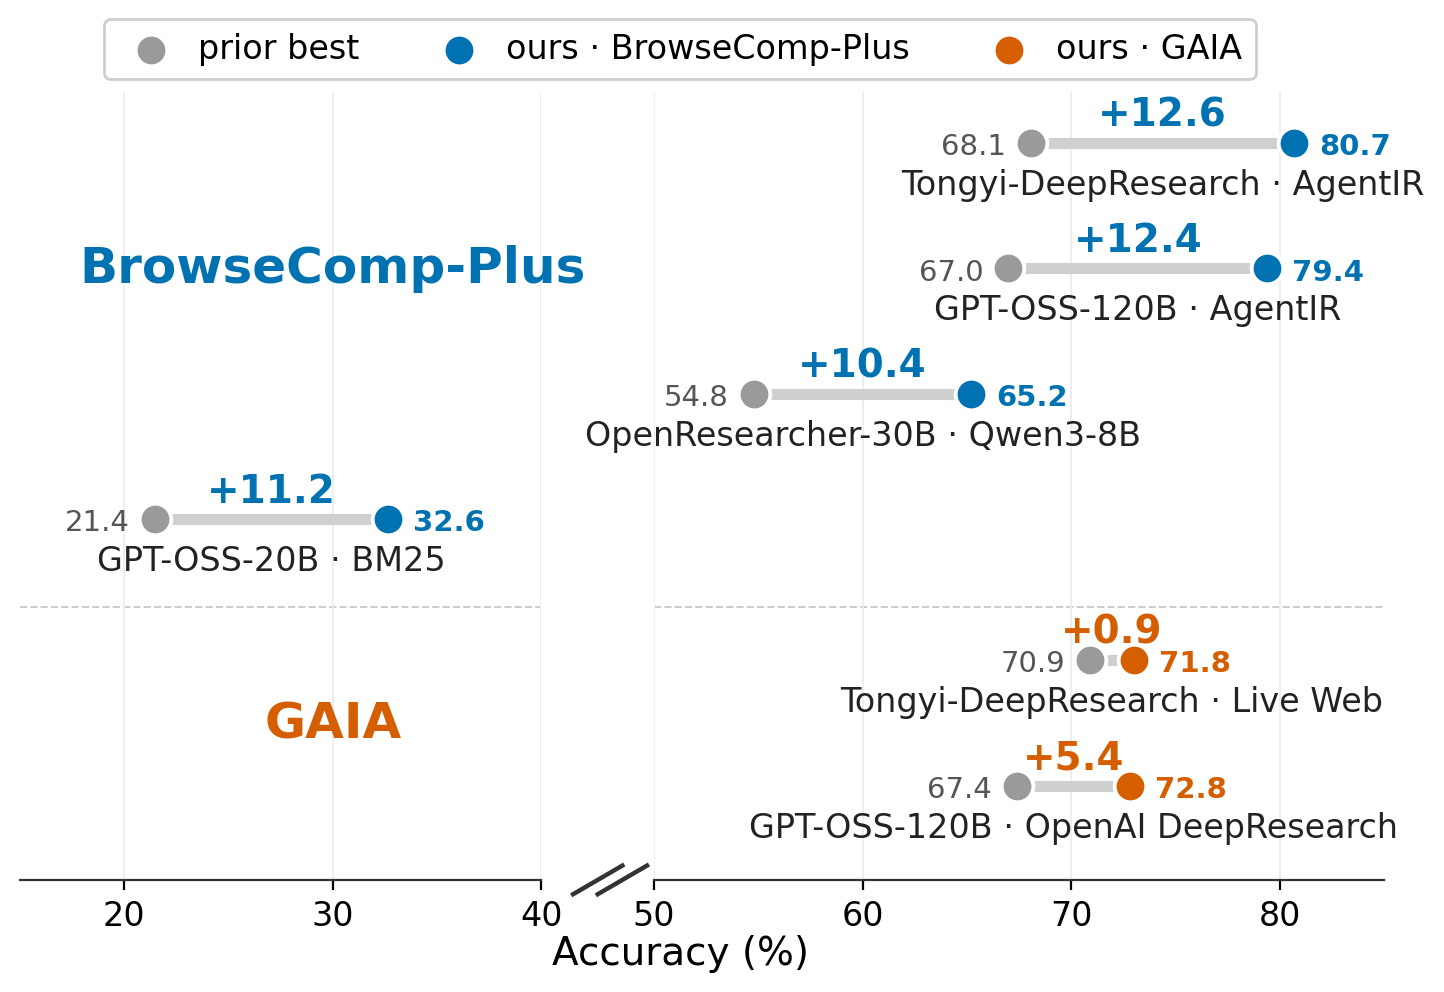
\includegraphics[width=\linewidth]{fig/reliability.png}
    \vspace{-2em}
    \caption{
Our scaffold consistently achieves higher \textit{No-CM} accuracy on BrowseComp-Plus and GAIA than the best publicly reported results for matched model--retriever pairs~\citep{chen2025browsecompplus,team2025tongyideepresearch,li2026openresearcher,chen2026agentir}.
% All results are reported as accuracy (\%).
}
\vspace{-3em}
\label{tab:scaffold-baseline}
\end{wrapfigure}
Before turning to the central question, \textit{when does observation masking help and why}, we first establish that the comparisons we will draw are made on a stronger baseline than previously available.

\paragraph{Higher baseline accuracy.}
Figure~\ref{tab:scaffold-baseline} compares the accuracy of our scaffold
(No-CM) against the highest publicly reported numbers for the same model--retriever pair on BrowseComp-Plus. Across the matched comparisons shown, our scaffold consistently improves accuracy (GPT-OSS-20B at $+$11.2 pts, GPT-OSS-120B at $+$12.4 pts, Tongyi-DeepResearch-30B-A3B at $+$12.6 pts). 


This stronger baseline matters for the analyses that follow. A weaker scaffold would inflate the apparent value of context management because any intervention that prunes noisy context can appear helpful when the agent is already failing due to scaffold deficiencies. By starting from stronger No-CM accuracy, our regime map (\S\ref{sec:results} and Table~\ref{tab:main}) measures the \emph{conservative} contribution of masking: the room for improvement on top of an already squeezed baseline.

